\chapter{}
\label{lecture9}
\section[Функционал Бесселя. Уравнение Бесселя (продолжение)]{Квадратичный функционал специального вида. Уравнение Бесселя (продолжение)}\markboth{Лекция~\thechapter.}{\thesection\quad Функционал Бесселя. Уравнение Бесселя}%
\label{lecture9section1}%
Итак{\mb,} рассматривая задачу на
\begin{multline*}
	\min\limits_{y\in\K}\J[y]\quad\text{для}\quad\J[y]=\int\limits_0^R\left(x\cdot y^{\prime2}+\frac{\nu^2}{x}\cdot y^2\right)\,dx,\\
	\K=\left\{y(x)\middle|y(x)\in\Cfn[{[0,R]}]{},\ y(R)=0,\vphantom{\int\limits_0^R}\right.\\\left. \begin{array}{rcl}
		\nu>0&:&y(0)=0,\ y\in\Cfn[{(0,R]}]{1},\\
		\nu=0&:&y\in\Cfn[{[0,R]}]{1},
	\end{array}\ \int\limits_0^R x\cdot y^2\,dx=1\right\},
\end{multline*} 
мы установили, что минимайзер должен удовлетворять уравнению
\begin{equation}\label{l9:eq:1}
	 Ly\eqdef-\der{}{x}\Big(x\cdot y'\Big)+\frac{\nu^2}{x}\cdot y=\lambda\cdot x\cdot y,
\end{equation}
то есть быть собственной функцией обобщённой задачи Штурма. Оператор $L$ рассматривается в области
\begin{multline*}
	\mc{D}_{L}=\left\{y(x)\middle|y\in\Cfn[{[0,R]}]{},\  y(R)=0,\vphantom{\begin{array}{rcl}
			\text{при }\nu=0&:&y\in\Cfn[{[0,R]}]{2},\\
			\text{при }\nu>0&:&y(0)=0,\ y\in\Cfn[{(0,R]}]{2},
	\end{array}}\right.\\\left. \begin{array}{rcl}
		\text{при }\nu=0&:&y\in\Cfn[{[0,R]}]{2},\\
		\text{при }\nu>0&:&y(0)=0,\ y\in\Cfn[{(0,R]}]{2},\ \norm{Ly}_1<+\infty,\ \J[y]<+\infty
	\end{array}\right\}.
\end{multline*}
Было установлено, что в этой области оператор $L$ --- эрмитов и 
\begin{equation}\label{l9:eq:2}
	\big(Ly,y\big)=\J[y].
\end{equation}
Из~\eqref{l9:eq:1} следует, что в скалярном произведении $(u,v)_1=\smallint\limits_0^R x\cdot u(x)\cdot\overline{v}(x)\,dx$ собственные функции обобщённой задачи Штурма, отвечающие различным собственным значениям{\mb,} ортогональны, а собственные значения~--- в силу~\eqref{l9:eq:2} --- неотрицательны, а при $\nu>0$ --- строго положительны, ибо в силу~\eqref{l9:eq:1},~\eqref{l9:eq:2}
\begin{equation}\label{l9:eq:3}
	\big(Ly,y\big)=\J[y]=\int\limits_0^R\left(x\cdot y^{\prime2}+\frac{\nu^2}{x}\cdot y^2\right)\,dx=\lambda\cdot\norm{y}_1^2.
\end{equation}   
Отметим, что при $\nu=0$ равенство $\lambda=0$ возможно лишь при $y'=0$, то есть при $y=const$, а так как $y(R)=0$, то $y\equiv0$. Значит, $\lambda>0$. Однако, если бы было другое граничное условие при $x=R$: $y'(R)=0$, то функция $y\equiv const$ и $\lambda=0$ были бы собственной функцией и собственным значением обобщённой задачи Штурма. Мы позже вернёмся к этому случаю, а пока считаем{\mb, что} $y(R)=0$ и{\mb,} значит{\mb,} $\lambda>0$. Так как оператор $L$ зависит от параметра $\nu$, то в~\eqref{l9:eq:1} мы будем писать $L=L(\nu)$, а решения~\eqref{l9:eq:1} и числа $\lambda$ обозначим через $y_{\nu k}$ и $\lambda_{\nu k}$, $k=1,2,\ldots$, где $\nu$ --- фиксировано, а $k$ нумерует собственные значения и собственные функции обобщённой задачи Штурма. Таким образом{\mb,}~\eqref{l9:eq:1} запишется в виде 
\begin{equation}\label{l9:eq:4}
	 L(\nu)y_{\nu k}=\lambda_{\nu k}\cdot x\cdot y_{\nu k}.
\end{equation}
Введём в~\eqref{l9:eq:4} новую независимую переменную $\rho\eqdef\sqrt{\lambda_{\nu k}}\cdot x$ и положим $z_{\nu k}(\rho)\equiv y_{\nu k}(x)$. Считаем $\nu$ и $k$ фиксированными{\mb;} у функции $z_{\nu k}(\rho)\?=z(\rho)$ эти индексы писать не будем. Легко видеть, что для функции $z(\rho)$ мы получим следующее уравнение:
\begin{equation}\label{l9:eq:5}
	\rho^2\cdot z''+\rho\cdot z'+\left(\rho^2-\nu^2\right)\cdot z=0,
\end{equation}
где в силу граничных условий и условий гладкости для функций $y_{\nu k}(x)$ мы должны потребовать
\begin{equation*}
	\begin{array}{lll}
		z(\sqrt{\lambda}\cdot R)=0,\quad&& z(\rho)\in\Cfn[{[0,R]}]{2}\ \text{при }\nu=0;\\[7pt] 
		z(\sqrt{\lambda}\cdot R)=0,\quad&z(0)=0,\quad& z(\rho)\in\Cfn[{(0,R]}]{2}\ \text{при }\nu>0.
	\end{array}
\end{equation*}

Уравнение~\eqref{l9:eq:5} хорошо известно. Это уравнение Бесселя, его решения --- функции Бесселя $\nu$-ого порядка. Так как уравнение~\eqref{l9:eq:5} --- уравнение второго порядка --- то оно имеет два линейно независимых решения, называемые функциями Бесселя первого и второго рода. Но функция Бесселя второго рода имеет особенность при $\rho=0$. Остаётся функция Бесселя первого рода $\nu$-ого порядка, или просто функция Бесселя $\nu$-ого порядка $J_\nu(\rho)$. Решение уравнения~\eqref{l9:eq:5} можно искать в виде ряда
\begin{equation*}
	\rho^{\nu}\cdot\sum\limits_{k=0}^{\infty}C_k^{(\nu)}\cdot\rho^k.
\end{equation*}  
После подстановки в~\eqref{l9:eq:5} получим, что 
\begin{equation}\label{l9:eq:6}
	 J_{\nu}(\rho)=\rho^{\nu}\cdot\sum\limits_{k=0}^{\infty}C_{2\cdot k}^{(\nu)}\cdot\rho^{2\cdot k},
\end{equation}
где $\displaystyle C_{2\cdot k}^{(\nu)}=-C_{2\cdot k-2}^{(\nu)}\cdot\frac{1}{4\cdot k\cdot(k+1)}$,$\quad k=1,2,\ldots$

\noindent Таким образом{\mb,} все коэффициенты выражаются через коэффициент $C_0^{(\nu)}$, который свободен\footnote{Решение определено с точностью до множителя.}.

Итак, решение~\eqref{l9:eq:5} --- это $z(\rho)=J_{\nu}(\rho)$. Так как $y_{\nu k}(R)=0$, то $z(\sqrt{\lambda}\cdot R)=0=J_{\nu}\left(\sqrt{\lambda}\cdot R\right)$. Обозначим через $\mu_{\nu k}$, $k=1,2,\ldots$ нули функции $J_{\nu}(\rho):\,J_{\nu}\left(\mu_{\nu k}\right)=0$. Тогда $\sqrt{\lambda_{\nu k}}\cdot R=\mu_{\nu k}$ и 
\begin{equation}\label{l9:eq:7}
	\lambda_{\nu k}=\left(\frac{\mu_{\nu k}}{R}\right)^2.
\end{equation}
Таким образом{\mb,} так как $\rho=\sqrt{\lambda}\cdot x${\mb,}
\begin{equation}\label{l9:eq:8}
	 y_{\nu k}(x)=z(\rho)=J_{\nu}\left(\frac{\mu_{\nu k}}{R}\cdot x\right)\footnotemark{}.
\end{equation}\footnotetext{Теперь, когда $y_{\nu k}(x)=z$ найдены, надо проверить неравенства $\J[y_{\nu k}]<+\infty$, $\norm{Ly_{\nu k}}_1<+\infty$, которые должны выполняться в $\mc{D}_L$. Мы это сделаем позже.}

Мы получили явный вид собственных функций $y_{\nu k}$ и собственных значений $\lambda_{\nu k}$ обобщённой задачи Штурма. Так как в выражения~\eqref{l9:eq:7},~\eqref{l9:eq:8} входят нули функции Бесселя $J_{\nu}(\rho)$, то проведём небольшое исследование тех точек $\mu_{\nu k}$, в которых $J_{\nu}\left(\mu_{\nu k}\right)=0$, то есть изучим~--- хотя бы поверхностно ---  свойства нулей функции Бесселя. Для этого воспользуемся известной асимптотикой функции Бесселя при больших $\rho$
\begin{equation}\label{l9:eq:1.9}
	\sqrt{\rho}\cdot J_{\nu}(\rho)=a_{\nu}\cdot\cos(\rho-b_\nu)+O\left(\frac{1}{\rho}\right),
\end{equation}
где $a_{\nu}>0$ --- некоторое число, $\displaystyle b_{\nu}=\frac{\pi}{4}+\frac{\pi\cdot\nu}{2}$. Отсюда видно, что при $\rho=\rho_k=\pi\cdot k+b_{\nu}$ выполняется
\begin{equation}\label{l9:eq:9}
	\sqrt{\rho_k}\cdot J_{\nu}(\rho_k)=(-1)^k\cdot a_{\nu}+O\left(\frac{1}{\rho_k}\right).
\end{equation}
Величины $J_{\nu}(\rho_k)$ и $J_{\nu}(\rho_{k+1})$ при больших $\rho$ имеют в силу~\eqref{l9:eq:9} разные знаки. И так как функция $J_{\nu}(\rho)$ непрерывна на отрезке $[\rho_k,\rho_{k+1}]$, на этом отрезке обязательно найдётся нечётное число точек, в которой $J_{\nu}(\rho)$ обращается в ноль. В тоже время, так как функция $J_{\nu}(\rho)$ --- аналитична на отрезке $[\rho_k,\rho_{k+1}]$ при $\rho_k>0$, то на этом отрезке \emph{не может быть бесконечного числа нулей\footnote{Можно доказать, что для больших значений $k$ на отрезке $[\rho_k,\rho_{k+1}]$ находится всего один нуль функции Бесселя. Идея доказательства состоит в следующем. Обозначим через $\Phi(\rho)$ левую часть~\eqref{l9:eq:1.9}. В силу~\eqref{l9:eq:1.9} функция $\Phi(\rho)$ --- а значит и функция Бесселя --- на этом отрезке может обращаться в ноль только там, где модуль косинуса мал, то есть в малой окрестности точки $d_k=\pi\cdot(k+1/2)+b_{\nu}$. Из формул~\eqref{l9:eq:1.9} и~\eqref{l9:eq:1.11} следует, что асимптотика для производной $\displaystyle\der{\Phi}{\rho}$ даётся правой частью формулы~\eqref{l9:eq:1.11}. Значит, в окрестности точки $d_k$ модуль $\displaystyle\der{\Phi}{\rho}$ близок к $a_{\nu-1}>0$ не зависимо от $k$. Поэтому в окрестности $d_k$ может быть только один ноль функции $\Phi(\rho)$ --- а значит и функции Бесселя, так как в противном случае в окрестности этой точки должны были бы существовать нули $\displaystyle\der{\Phi}{\rho}$, а их --- нет.}}. Это относится вообще к любому отрезку $[\alpha,\beta]$ при $\alpha>0$. Что касается отрезка $[0,\alpha]$, то в силу~\eqref{l9:eq:6} при $0<\alpha<1$
\begin{equation*}
	 J_{\nu}(\rho)=\rho^{\nu}\cdot\Big(C_0^{(\nu)}+O(\rho)\Big)\quad\text{при}\quad\rho\ll1.
\end{equation*}
Следовательно, нули $\mu_{\nu k}$ функции $J_{\nu}(\rho)$ могут накапливаться только на бесконечности. Поэтому при $k\to\infty$ собственные значения $\lambda_{\nu k}\?=\left(\mu_{\nu k}/R\right)^2\to\infty$. Таким образом{\mb,} мы получили бесконечную последовательность при $k\to\infty$ собственных функций обобщённой задачи Штурма
\begin{equation*}
	 y_{\nu k}(x)=J_{\nu}\left(\frac{\mu_{\nu k}}{R}\cdot x\right),
\end{equation*}
отвечающих собственным значениям 
\begin{equation*}
	 \lambda_{\nu k}=\left(\frac{\mu_{\nu k}}{R}\right)^2\to\infty,\quad\text{при}\quad k\to\infty.
\end{equation*}
В силу свойств решений обобщённой задачи Штурма 
\begin{equation*}
	\big(y_{\nu k},y_{\nu m}\big)_1=\left(J_{\nu}\left(\frac{\mu_{\nu k}}{R}\cdot x\right),J_{\nu}\left(\frac{\mu_{\nu m}}{R}\cdot x\right)\right)_1=0,\quad k\neq m.
\end{equation*}
\begin{Teor}[теорема Стеклова]
	Пусть
	\begin{equation*}
		 d_k^{(\nu)}\eqdef\left(y,J_{\nu}\left(\frac{\mu_{\nu k}}{R}\cdot x\right)\right)_1\Biggm/\norm{J_{\nu}\left(\frac{\mu_{\nu k}}{R}\cdot x\right)}_1^2.
	\end{equation*} 
	Тогда 
	\begin{enumerateP1}
		\item\label{l9:Steclov:L}при $y\in\fLr[{[0,R];x}]$\quad $\displaystyle\norm{y-\sum\limits_{k=1}^{n}d_k^{(\nu)}\cdot J_{\nu}\left(\frac{\mu_{\nu k}}{R}\cdot x\right)}_1\to0$ при $n\to\infty$,
		\item\label{l9:Steclov:D}при $y\in\mc{D}_L$\quad$\displaystyle\sup\limits_{x\in[a,b]}\left|y-\sum\limits_{k=1}^{n}d_k^{(\nu)}\cdot J_{\nu}\left(\frac{\mu_{\nu k}}{R}\cdot x\right)\right|\to0$ при $n\to\infty$. 
	\end{enumerateP1} 
\end{Teor}
\noindent\ref{l9:Steclov:D} --- без доказательства, а \ref{l9:Steclov:L} --- доказать самостоятельно при $y\?\in\mc{D}_L$. 

Рассмотрим теперь случай граничного условия $y'(R)=0$ вместо $y(R)=0$. Обозначим соответствующие собственные функции и собственные значения обобщённой задачи Штурма через $\tilde{y}_{\nu k}(x)$ и через $\tilde{\lambda}_{\nu k}$. Вводим функцию $\tilde{z}(\rho)=\tilde{y}_{\nu k}(x)$, где $\rho=\sqrt{\tilde{\lambda}_{\nu k}}\cdot x$. Для функции $\tilde{z}(\rho)$ мы{\mb,} как и раньше{\mb,} получим уравнение Бесселя, выберем нужное нам решение $J_{\nu}(\rho)$, но теперь граничное условие при $x=R$, то есть при $\rho=\sqrt{\tilde{\lambda}}\cdot R${\mb,} будет $J_{\nu}'\left(\sqrt{\tilde{\lambda}}\cdot R\right)=0$. Обозначим нули функции $J_{\nu}'(\rho)$ через $\tilde{\mu}_{\nu k}$ и тогда 
\begin{equation*}
	\tilde{\lambda}_{\nu k}=\left(\frac{\tilde{\mu}_{\nu k}}{R}\right)^2,\quad \tilde{y}_{\nu k}(x)=J_{\nu}\left(\frac{\tilde{\mu}_{\nu k}}{R}\cdot x\right).
\end{equation*}
Чтобы убедит{\mbь}ся в существовании бесконечного числа нулей $\tilde{\mu}_{\nu k}$ функции $J_{\nu}'(\rho)${\mb,} рассмотрим её асимптотику при $\rho\gg1$
\begin{equation}\label{l9:eq:1.11}
	\sqrt{\rho}\cdot J_{\nu}'(\rho)=a_{\nu-1}\cdot\sin(\rho-b_{\nu})+O\left(\frac{1}{\rho}\right){\mb,}
\end{equation}
и {\mbбудем действовать} аналогично предыдущему. Дальнейшее рассмотрение обобщённой задачи Штурма с изменённым граничным условием не отличается от рассмотрения задачи с граничным условием $y(R)=0$.

Теперь проверим, что функции $y_{\nu k}\in\mc{D}_L$. Нам осталось проверить два утверждения: $\J[y_{\nu k}]\?<+\infty$ и $\norm{Ly_{\nu k}}_1<+\infty$ ($\nu>0$). В силу~\eqref{l9:eq:6} и~\eqref{l9:eq:8} можно записать
\begin{equation*}
	 y_{\nu k}(x)=x^{\nu}\cdot\Phi(x), 
\end{equation*}
где, конечно, $\Phi(x)=\Phi_{\nu k}(x)$, но у нас $\nu$ и $k$ --- фиксированы и мы опускаем эти индексы. $\Phi(x)$ --- бесконечно дифференцируема на $[0,+\infty)$. Найдём $y_{\nu k}'$ и $y_{\nu k}''${\mb:}
\begin{gather*}
	 y_{\nu k}'=\nu\cdot x^{\nu-1}\cdot\Phi(x)+x^{\nu}\cdot\Phi'(x),\\ y_{\nu k}''=\nu\cdot(\nu-1)\cdot x^{\nu-2}\cdot\Phi(x)+2\cdot\nu\cdot x^{\nu-1}\cdot\Phi'(x)+x^{\nu}\cdot\Phi''(x).
\end{gather*}
Очевидно,
\begin{equation*}
	 x\cdot y_{\nu k}^{\prime2}\leqslant const\cdot\left(x^{2\cdot\nu}\cdot\Phi^{\prime2}(x)\cdot x+x^{2\cdot\nu}\cdot|\Phi(x)|\cdot|\Phi'(x)|+x^{2\cdot\nu-1}\cdot\Phi^2(x)\right).
\end{equation*}
Так как $\nu>0$, то
\begin{equation*}
	\int\limits_0^R\left(x\cdot y_{\nu k}^{\prime2}+\frac{\nu^2}{x}\cdot y_{\nu k}^2\right)\,dx<+\infty
\end{equation*}
и 
\begin{equation*}
	\norm{Ly_k}_1^2=\int\limits_0^R x\cdot\left[-\der{}{x}\left(x\cdot y_{\nu k}'\right)+\frac{\nu^2}{x}\cdot y_{\nu k}\right]^2\,dx<+\infty.
\end{equation*}
то есть $y_{\nu k}\in\mc{D}_L$. 

Но можно было проще: $Ly_{\nu k}=x\cdot\lambda_{\nu k}\cdot y_{\nu k}$ и{\mb,} значит{\mb,}
\begin{equation*}
	\norm{Ly_{\nu k}}_1^2=\lambda_{\nu k}^2\cdot\norm{x\cdot y_{\nu k}}_1^2=\lambda_{\nu k}^2\cdot\int\limits_0^R x^3 y_{\nu k}^2\,dx<+\infty.
\end{equation*} 
\section[Функционалы, зависящие от функций двух переменных]{Вариационные задачи для функционалов, зависящих от функций двух переменных}
\label{lecture9section2}
Рассмотрим следующую задачу. Пусть дана цилиндрическая ёмкость с образующими{\mb,} параллельными оси $z$. В плоскости $x,\ y$ <<дно>> этой ёмкости образует какую-то область $G$. Сверху ёмкость не закрыта, граница цилиндрической поверхности сверху --- функция $f(x,y)$, $x,y\in\partial G$ ($\partial G$ --- граница $G$).


\begin{figure}[H]\centering
\tikzset{every picture/.style={line width=0.75pt}} %set default line width to 0.75pt        

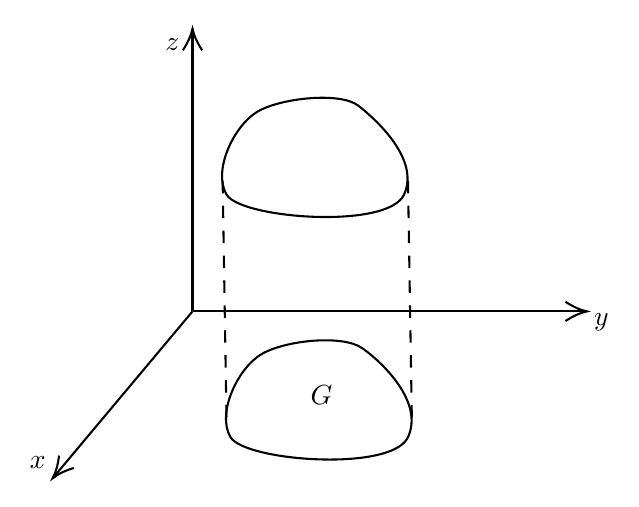
\begin{tikzpicture}[x=0.75pt,y=0.75pt,yscale=-0.95,xscale=0.95]
	%uncomment if require: \path (0,250); %set diagram left start at 0, and has height of 250
	
	%Straight Lines [id:da7533107082747501] 
	\draw    (216.72,146.22) -- (414.78,146.22) ;
	\draw [shift={(416.78,146.22)}, rotate = 180] [color={rgb, 255:red, 0; green, 0; blue, 0 }  ][line width=0.75]    (10.93,-4.9) .. controls (6.95,-2.3) and (3.31,-0.67) .. (0,0) .. controls (3.31,0.67) and (6.95,2.3) .. (10.93,4.9)   ;
	%Straight Lines [id:da9386510837032684] 
	\draw    (216.72,146.22) -- (147.07,229.32) ;
	\draw [shift={(145.78,230.85)}, rotate = 309.97] [color={rgb, 255:red, 0; green, 0; blue, 0 }  ][line width=0.75]    (10.93,-4.9) .. controls (6.95,-2.3) and (3.31,-0.67) .. (0,0) .. controls (3.31,0.67) and (6.95,2.3) .. (10.93,4.9)   ;
	%Straight Lines [id:da22581012210637597] 
	\draw    (216.72,146.22) -- (216.72,4.85) ;
	\draw [shift={(216.72,2.85)}, rotate = 450] [color={rgb, 255:red, 0; green, 0; blue, 0 }  ][line width=0.75]    (10.93,-4.9) .. controls (6.95,-2.3) and (3.31,-0.67) .. (0,0) .. controls (3.31,0.67) and (6.95,2.3) .. (10.93,4.9)   ;
	%Shape: Polygon Curved [id:ds441803632619425] 
	\draw   (251.78,167.85) .. controls (263.78,160.85) and (292.78,157.85) .. (302.78,164.85) .. controls (312.78,171.85) and (334.22,192.15) .. (326,210) .. controls (317.78,227.85) and (243.22,222.15) .. (236,210) .. controls (228.78,197.85) and (239.78,174.85) .. (251.78,167.85) -- cycle ;
	%Shape: Polygon Curved [id:ds2324963963699278] 
	\draw   (249.78,44.85) .. controls (261.78,37.85) and (291.78,34.85) .. (300.78,41.85) .. controls (309.78,48.85) and (332.22,69.15) .. (324,87) .. controls (315.78,104.85) and (241.22,99.15) .. (234,87) .. controls (226.78,74.85) and (237.78,51.85) .. (249.78,44.85) -- cycle ;
	%Straight Lines [id:da6083220832384053] 
	\draw  [dash pattern={on 4.5pt off 4.5pt}]  (232,80) -- (234,203) ;
	%Straight Lines [id:da7239634925795717] 
	\draw  [dash pattern={on 4.5pt off 4.5pt}]  (326,80) -- (328,203) ;
	
	% Text Node
	\draw (211.72,6.25) node [anchor=north east] [inner sep=0.75pt]    {$z$};
	% Text Node
	\draw (143.78,227.45) node [anchor=south east] [inner sep=0.75pt]    {$x$};
	% Text Node
	\draw (418.78,145.62) node [anchor=north west][inner sep=0.75pt]    {$y$};
	% Text Node
	\draw (275,182.4) node [anchor=north west][inner sep=0.75pt]    {$G$};
	
\end{tikzpicture}
	\caption{}
\label{l9:fig:1}
\end{figure}

\noindent\textbf{Задача:} закрыть цилиндр крышкой наименьшей площади. Если обозначить закрывающую поверхность через $z(x,y)$, то площадь крышки
\begin{equation*}
	 S[z]=\iint\limits_{G}\sqrt{1+z_x^2+z_y^2}\,dxdy,
\end{equation*}
и мы должны минимизировать функционал $S[z]$ в классе функций $z(x,y)$, $z\Big|_{\partial G}=f(x,y)$, $z\?\in\Cfn[]{1}(G)$.

Перейдём теперь к общему случаю. Вводим обозначения $p\eqdef\displaystyle\pder{z}{x}$, $q\eqdef\displaystyle\pder{z}{y}$. Рассмотрим функционал
\begin{equation*}
	\J[z]=\iint\limits_{G}F(x,y,z,p,q)\,dxdy,
\end{equation*}
где $G$ --- некоторая область в плоскости $x,\ y$, $F\in\Cfn{2}$ при $(x,y)\in G$, $|z|\?<M$, $\forall p,\ q$; здесь $M$ --- какая-то большая константа. Пусть $P\eqdef(x,y)$. И пусть
\begin{equation*}
	\K\eqdef\left\{z(x,y)\middle|z\in\Cfn{1}(\overline{G}),\ z\Big|_{\partial G}=f(P),\ |z|<M\right\}.
\end{equation*}
Мы будем рассматривать задачу на $\displaystyle\min\limits_{z\in\K}\,\J[z]$. Как обычно{\mb,} предполагаем, что минимайзер существует и обладает повышенной гладкостью. Пусть $z=z(x,y)$ --- минимайзер в рассматриваемой задаче.
\begin{Def}
	Функцию $\eta(x,y)$ назовём \textbf{допустимым изменением}, если $\tilde{z}\eqdef z+t\cdot\eta\in\K$ при $|t|\ll1$.
\end{Def}  
Легко видеть, что отсюда вытекают такие ограничения на $\eta$: $\eta\Big|_{\partial G}\?=0$, $\eta\in\Cfn{1}(\overline{G})$. Далее проводим стандартные рассуждения. Полагаем $\phi(t)=\J[z+t\cdot\eta]$. Тогда
\begin{equation*}
	\J[z+t\cdot\eta]\geqslant\J[z]\quad\Rightarrow\quad\phi(t)\geqslant\phi(0);
\end{equation*}
\begin{equation*}
	\J[z+t\cdot\eta]-\J[z]=\delta\J+\ldots,\qquad\phi(t)-\phi(0)=\phi'(0)\cdot t+\ldots;
\end{equation*}
\begin{equation*}
	\delta\J=t\cdot\phi'(0)=t\cdot\left.\der{}{t}\J[z+t\cdot\eta]\right|_{t=0}\ \text{--- первая вариация.}
\end{equation*}
Так как $\phi(0)$ --- минимальное значение $\phi(t)$ при $|t|\ll1$, то $\phi'(0)=0$ (функция $\phi(t)\in\Cfn{1}$!), то есть $\delta\J=0$ --- необходимое условие минимума (для максимума --- тоже). Вычислим первую вариацию функционала 
\begin{equation*}
	\J[z+t\cdot\eta]=\iint\limits_{G}\overbrace{F(x,y,\underbrace{z+t\cdot\eta}_{\tilde{z}},\underbrace{p+t\cdot\eta_x}_{\tilde{z}_x},\underbrace{q+t\cdot\eta_y}_{\tilde{z}_y})}^{\widetilde{F}}\,dxdy.
\end{equation*}
Имеем (предполагая только $z\in\Cfn{2}$, $\eta\in\Cfn{1}$)
\begin{multline*}
	\delta\J=\left.t\cdot\der{}{t}\iint\limits_{G}\widetilde{F}\,dxdy\right|_{\lefteqn{\scriptstyle t=0}}=\left.t\cdot\iint\limits_{G}\left(\widetilde{F}_{\tilde{z}}\cdot\eta+\widetilde{F}_{\tilde{z}_x}\cdot\eta_x+\widetilde{F}_{\tilde{z}_y}\cdot\eta_y\right)\,dxdy\right|_{\lefteqn{\scriptstyle t=0}}=\\=t\cdot\iint\limits_{G}\left({F}_{z}\cdot\eta+{F}_{z_x}\cdot\eta_x+{F}_{z_y}\cdot\eta_y\right)\,dxdy.
\end{multline*}
Преобразуем полученное выражение так, чтобы производные $\eta_x$ и $\eta_y$ входили только в выражение дивергенции некоторого вектора. Имеем
\begin{multline*}
	\iint\limits_{G}\left(F_p\cdot\eta_x+F_q\cdot\eta_y\right)\,dxdy=\iint\limits_{G}\left(\der{}{x}(F_p\cdot\eta)+\der{}{y}(F_q\cdot\eta)\right)\,dxdy-\\-\iint\limits_{G}\left(\der{}{x}F_p+\der{}{y}F_q\right)\cdot\eta\,dxdy.
\end{multline*}
Таким образом, первая вариация
\begin{multline*}
	\delta\J=t\left[\iint\limits_{G}\left(F_z-\der{}{x}F_p-\der{}{y}F_q\right)\cdot\eta\,dxdy+\right.\\\left.+\iint\limits_{G}\left(\der{}{x}(F_p\cdot\eta)+\der{}{y}(F_q\cdot\eta)\right)\,dxdy\right].
\end{multline*}
Введём в рассмотрение вектор $\bm{\Phi}=(F_p\cdot\eta,F_q\cdot\eta)$. Его компоненты обладают гладкостью $\Cfn{1}(G)$ и $\Cfn{}(\overline{G})$. Поэтому можно применить формулу Остроградского--Гаусса, согласно которой
\begin{center}
	\fbox{$\displaystyle\iint\limits_{G}\Div\bm{\Phi}\,dxdy=\int\limits_{\partial G}\big(\bm{\Phi},\bm{n}\big)_{\R^2}\,dl,$}
\end{center}
где $\bm{n}=(\cos\alpha,\cos\beta)$ --- единичная внешняя нормаль к границе $\partial G$.

\noindent Используя эту формулу{\mb,} получаем окончательное выражение для первой вариации{\mb:}
\begin{multline}\label{l9:eq:10}
	\delta\J=t\cdot\iint\limits_{G}\left(F_z-\der{}{x}F_p-\der{}{y}F_q\right)\cdot\eta\,dxdy+\\+t\cdot\int\limits_{\partial G}(F_p\cdot\cos\alpha+F_q\cdot\cos\beta)\cdot\eta\,dl.
\end{multline}

Заметим, что это выражение даёт главную {\mb часть } приращения $\J[{z+t\cdot\eta}]-\J[z]$ независимо ни от каких свойств $z$ и $\eta${\mb,} кроме гладкости. Мы этим будем пользоваться.

Теперь возвращаемся к нашей вариационной задаче. Если $z$ --- минимайзер и $\eta$ --- допустимое изменение, то $\eta\Big|_{\partial G}\equiv0$ и $\delta\J=0$, то есть
\begin{equation}\label{l9:eq:11}
	\iint\limits_{G}\left(F_z-\der{}{x}F_p-\der{}{y}F_q\right)\cdot\eta\,dxdy=0,\quad\forall\eta\text{ --- допустимое.}
\end{equation}
Пусть $\displaystyle\Psi\equiv F_z-\der{}{x}F_p-\der{}{y}F_q$. Тогда~\eqref{l9:eq:11} означает, что 
\begin{equation}\label{l9:eq:12}
	\iint\limits_{G}\Psi(x,y)\cdot\eta\,dxdy=0,\quad\forall\eta\text{ --- допустимое.}
\end{equation}
Из равенства~\eqref{l9:eq:12} вытекает, что $\Psi(x,y)\equiv0$, $x,y\in G$ (обобщение леммы Лагранжа на плоскость). Действительно, пусть в некоторой точке $x_0,y_0$ выполняется $\Psi(x_0,y_0)>0$. Так как функция $\Psi(x,y)$~--- непрерывная, то можно указать такой квадрат $A$ со стороной $2\cdot\delta$: $|x-x_0|\leqslant\delta$, $|y-y_0|\leqslant\delta$, что $\Psi(x,y)>0$, $x,y\in A$.

\begin{figure}[H]\centering
\tikzset{every picture/.style={line width=0.75pt}} %set default line width to 0.75pt        

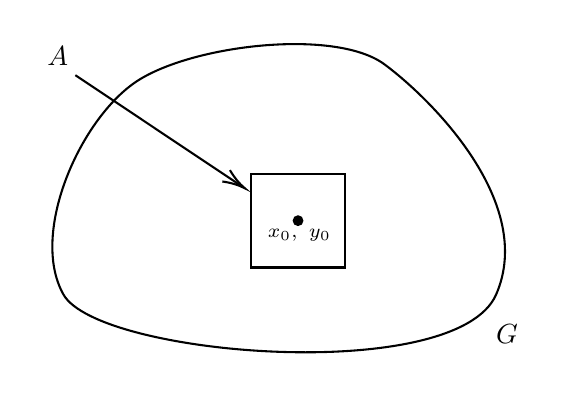
\begin{tikzpicture}[x=0.75pt,y=0.75pt,yscale=-1,xscale=1]
	%uncomment if require: \path (0,199); %set diagram left start at 0, and has height of 199
	
	%Shape: Polygon Curved [id:ds8647161812959627] 
	\draw   (71.59,37) .. controls (99.39,19.82) and (166.58,12.45) .. (189.74,29.64) .. controls (212.91,46.82) and (262.56,96.65) .. (243.53,140.48) .. controls (224.49,184.32) and (51.75,170.3) .. (35.03,140.48) .. controls (18.31,110.66) and (43.79,54.19) .. (71.59,37) -- cycle ;
	%Shape: Circle [id:dp30365118515163947] 
	\draw  [fill={rgb, 255:red, 0; green, 0; blue, 0 }  ,fill opacity=1 ] (146,104.93) .. controls (146,103.78) and (146.93,102.85) .. (148.07,102.85) .. controls (149.22,102.85) and (150.15,103.78) .. (150.15,104.93) .. controls (150.15,106.07) and (149.22,107) .. (148.07,107) .. controls (146.93,107) and (146,106.07) .. (146,104.93) -- cycle ;
	%Shape: Square [id:dp9936568887522785] 
	\draw   (125.52,82.38) -- (170.62,82.38) -- (170.62,127.48) -- (125.52,127.48) -- cycle ;
	%Straight Lines [id:da11258115446689132] 
	\draw    (40.78,34.85) -- (120.86,88.27) ;
	\draw [shift={(122.52,89.38)}, rotate = 213.7] [color={rgb, 255:red, 0; green, 0; blue, 0 }  ][line width=0.75]    (10.93,-3.29) .. controls (6.95,-1.4) and (3.31,-0.3) .. (0,0) .. controls (3.31,0.3) and (6.95,1.4) .. (10.93,3.29)   ;
	
	% Text Node
	\draw (242,153.4) node [anchor=north west][inner sep=0.75pt]    {$G$};
	% Text Node
	\draw (132,107.4) node [anchor=north west][inner sep=0.75pt]  [font=\scriptsize]  {$x_{0} ,\ y_{0}$};
	% Text Node
	\draw (38.78,31.45) node [anchor=south east] [inner sep=0.75pt]    {$A$};
	
	
\end{tikzpicture}
	\caption{}
\label{l9:fig:2}
\end{figure}
\noindent Определим функцию $\eta(x,y)$ равенствами 
\begin{multline*}
	\eta(x,y)=\\=\begin{cases}
		\left[(x-x_0+\delta)^2\!\cdot\!(x-x_0-\delta)^2\!\cdot\!(y-y_0+\delta)^2\!\cdot\!(y-y_0-\delta)^2\right]&\!\!x,y\in A,\\
		0&\!\!x,y\notin A.
	\end{cases}
\end{multline*}
Ясно, что по определению $\eta\Big|_{\partial A}=0$ и $\displaystyle\pder{\eta}{x}=\pder{\eta}{y}=0$, $x,y\in\partial A$. Поэтому нет разрывов функции $\eta$ и её производных на $\partial A$ и{\mb,} значит{\mb,} $\eta\in\Cfn{1}(\overline{G})$. Подставляя в~\eqref{l9:eq:11}{\mb,} получим
\begin{equation*}
	\iint\limits_{A}\Psi(x,y)\cdot\eta(x,y)\,dxdy=0,
\end{equation*}
что невозможно, ибо в области $A$ функции $\Psi(x,y)$ и $\eta(x,y)$ --- положительны (кроме границы). Значит, не может существовать такая точка $x_0,y_0$ в которой $\Psi(x_0, y_0)>0$. Аналогично убеждаемся, что не может быть точки $x_0,y_0$, в которой $\Psi(x_0,y_0)<0$. Значит $\Psi(x,y)\equiv0$, то есть
\begin{equation*}
	 F_z-\der{}{x}F_p-\der{}{y}F_q\equiv0{\mb,}
\end{equation*}
если в функцию $F(x,y,z,p,q)$ подставили минимайзер, то есть для нахождения минимайзера надо решить уравнение
\begin{equation}\label{l9:eq:13}
	 F_z-\der{}{x}F_p-\der{}{y}F_q=0.
\end{equation}
Это --- \textbf{уравнение Остроградского}. Мы должны решать его в классе функций $z(x,y)\in\Cfn{2}(G)$, $z\Big|_{\partial G}=f(x,y)$.

Уравнение~\eqref{l9:eq:13} --- это уравнение в частных производных второго порядка. Проведя в~\eqref{l9:eq:13} дифференцирование, получим
\begin{multline*}
	F_z-F_{px}-F_{pz}\cdot\pder{z}{x}-F_{pp}\cdot\pdder{z}{x}-F_{pq}\cdot\pder{^2z}{x\partial y}-F_{qy}-F_{qz}\cdot\pder{z}{y}-\\-F_{qp}\cdot\pder{^2z}{x\partial y}-F_{qq}\cdot\pdder{z}{y}=0,
\end{multline*}
то есть
\begin{equation}\label{l9:eq:14}
	-F_{pp}\cdot\pdder{z}{x}-2\cdot F_{pq}\cdot\pder{^2z}{x\partial y}-F_{qq}\cdot\pdder{z}{y}=W(x,y,z,p,q).
\end{equation}

Рассмотрим пример. Интеграл

\begin{equation*}
	\J[z]=\iint\limits_{G}\left[\left(\pder{z}{x}\right)^2+\left(\pder{z}{y}\right)^2\right]\,dxdy=\iint\limits_{G}\left(p^2+q^2\right)\,dxdy
\end{equation*}
называется интегралом Дирихле. Уравнение Остроградского для него 
\begin{equation*}
	-\der{}{x}(2\cdot z_x)-\der{}{y}(2\cdot z_y)=0,
\end{equation*}
то есть
\begin{equation*}
	\pdder{z}{x}+\pdder{z}{y}=0\text{ --- уравнение Лапласа},
\end{equation*}
оператор $\displaystyle\Delta\eqdef\pdder{}{x}+\pdder{}{y}$ --- оператор Лапласа.

\noindent\underline{Обобщение}. Рассмотрим функционал $\J[z]$ для функции $z\?=z(x_1,\ldots,x_n)$, зависящей от $n$ переменных. Пусть $\displaystyle p_i\eqdef\pder{z}{x_i}$, $i=\overline{1,n}$, $\Omega=\{x_1,\ldots,x_n\}$ --- некоторая область,
\begin{equation*}
	\J[z]=\idotsint\limits_{\Omega}F(x_1,\ldots,x_n,z,p_1,\ldots,p_n)\,d\Omega
\end{equation*}
и $z\Big|_{\partial\Omega}=f(x_1,\ldots,x_n)$. Уравнение Остроградского для этого функционала выводится совершенно аналогично случаю $n=2$. В результате мы получим 
\begin{equation*}
	 F_z-\der{}{x_1}F_{p_1}-\der{}{x_2}F_{p_2}-\ldots-\der{}{x_n}F_{p_n}=0.
\end{equation*}
\section{Вариационные задачи со свободной границей}
\label{lecture9section3}
Возвращаемся к исходному функционалу
\begin{equation*}
	\J[z]=\iint\limits_{G}F(x,y,z,p,q)\,dxdy,
\end{equation*}
но класс допустимых функций в задаче на $\min\,\J[z]$ определим по-другому. Пусть кривая $\Gamma\eqdef\partial G$. Разобьём $\Gamma$ произвольным образом на две части $\Gamma=\Gamma_1\cup \Gamma_2$, причём 
\begin{enumerate}
	\item одна из частей может отсутствовать,
	\item кривые $\Gamma_1$ и $\Gamma_2$ могут состоять каждая из отдельных кусков (см.~рис.~\ref{l9:fig:3}, например; $\Gamma_1$ выделена жирным).
\end{enumerate} 
\begin{figure}[H]\centering
\tikzset{every picture/.style={line width=0.75pt}} %set default line width to 0.75pt        

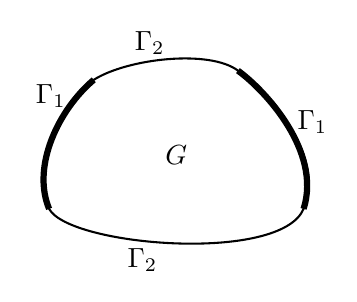
\begin{tikzpicture}[x=0.75pt,y=0.75pt,yscale=-0.7,xscale=0.7]
	%uncomment if require: \path (0,187); %set diagram left start at 0, and has height of 187
	
	%Shape: Polygon Curved [id:ds8076294015434553] 
	\draw   (63.89,42.58) .. controls (87.24,27.83) and (143.68,21.5) .. (163.14,36.26) .. controls (182.6,51.02) and (224.31,93.79) .. (208.32,131.42) .. controls (192.33,169.06) and (47.22,157.03) .. (33.18,131.42) .. controls (19.13,105.82) and (40.54,57.34) .. (63.89,42.58) -- cycle ;
	%Curve Lines [id:da5463349166005875] 
	\draw [line width=2.25]    (163.14,36.26) .. controls (181.89,49.86) and (220.89,91.86) .. (208.32,131.42) ;
	%Curve Lines [id:da42261145901201513] 
	\draw [line width=2.25]    (33.18,131.42) .. controls (20.89,101.86) and (39.89,62.86) .. (63.89,42.58) ;
	
	% Text Node
	\draw (111,85.4) node [anchor=north west][inner sep=0.75pt]    {$G$};
	% Text Node
	\draw (202,61.4) node [anchor=north west][inner sep=0.75pt]    {$\Gamma _{1}$};
	% Text Node
	\draw (22,43.4) node [anchor=north west][inner sep=0.75pt]    {$\Gamma _{1}$};
	% Text Node
	\draw (85,156.4) node [anchor=north west][inner sep=0.75pt]    {$\Gamma _{2}$};
	% Text Node
	\draw (90,7.4) node [anchor=north west][inner sep=0.75pt]    {$\Gamma _{2}$};
	
	
\end{tikzpicture}
	\caption{}
\label{l9:fig:3}
\end{figure}
Причина подобного разбиения --- необходимость описать ситуацию, когда часть границы --- скажем $\Gamma_2$ --- свободна, а на $\Gamma_1$ задано граничное условие (до сих пор $\Gamma_2=\varnothing$).

Итак, определим класс допустимых функций
\begin{equation*}
	\K=\left\{z(x,y)\middle|z\in\Cfn{1}(\overline{G}),\ z\Big|_{\Gamma_1}=f(x,y),\ \Gamma_2\neq\varnothing,\ |z|<M\right\}.
\end{equation*}  
Тогда, чтобы $z+t\cdot\eta\in\K${\mb,} нам необходимо требовать, чтобы $\eta(x,y)\equiv0$ не на всей кривой $\Gamma=\partial G$, а только на $\Gamma_1$. Достаточно условия: $\eta\Big|_{\Gamma_1}\equiv0$, а $\eta\Big|_{\Gamma_2}$ --- произвольна. Разумеется, требование $\eta(x,y)\in\Cfn{1}(\overline{G})$ --- сохраняется. Если $z$ --- минимайзер, то $\delta\J=0$, а формула для $\delta\J$ --- это~\eqref{l9:eq:10}. Значит{\mb,}
\begin{multline*}
	\delta\J=t\left[\iint\limits_{G}\left(F_z-\der{}{x}F_p-\der{}{y}F_q\right)\cdot\eta\,dxdy+\right.\\\left.+\int\limits_{\Gamma}\left(F_p\cdot\cos\alpha+F_q\cdot\cos\beta\right)\cdot\eta\,dl\right]=0.
\end{multline*}
Взяв $\eta\Big|_{\Gamma}\equiv0$ (это не запрещено){\mb,} мы получаем, что
\begin{equation*}
	\iint\limits_{G}\left(F_z-\der{}{x}F_p-\der{}{y}F_q\right)\cdot\eta\,dxdy=0,
\end{equation*}
откуда{\mb,} как и раньше{\mb,} выводим уравнение Остроградского
\begin{equation*}
	 F_z-\der{}{x}F_p-\der{}{y}F_q=0.
\end{equation*}
Поэтому равенство $\delta\J=0$ сводится к равенству
\begin{equation*}
	\int\limits_{\Gamma}(F_p\cdot\cos\alpha+F_q\cdot\cos\beta)\cdot\eta\,dl=0,\quad\forall\eta\text{ --- допустимое.}
\end{equation*}
Но так как $\eta\Big|_{\Gamma_1}\equiv0$, а $\Gamma=\Gamma_1\cup\Gamma_2$, то мы получаем, что
\begin{equation}\label{l9:eq:15}
	\int\limits_{\Gamma_2}(F_p\cdot\cos\alpha+F_q\cdot\cos\beta)\cdot\eta\,dl=0.
\end{equation}
В силу произвольности функции $\eta$ на $\Gamma_2$ мы, обобщая лемму Лагранжа на случай кривой, получим, что
\begin{equation}\label{l9:eq:16}
	 F_p\cdot\cos\alpha+F_q\cdot\cos\beta=0,\quad(x,y)\in\Gamma_2.
\end{equation}
Это --- естественное граничное условие для свободной части границы. Если $\Gamma_1=\varnothing$, то условие~\eqref{l9:eq:16} должно выполняться на всей границе $\Gamma=\partial G$. Таким образом{\mb,} уравнение Остроградского надо решать с граничными условиями: на $\Gamma_2$ ---~\eqref{l9:eq:16}, $z\Big|_{\Gamma_1}=f(x,y)$.

Приведём пример. Пусть $F=z_x^2+z_y^2$, то есть мы рассматриваем интеграл Дирихле. Тогда \begin{equation*}
	F_p\cdot\cos\alpha+F_q\cdot\cos\beta=2\cdot(z_x\cdot\cos\alpha+z_y\cdot\cos\beta)=2\cdot\big(\nabla z,\bm{n}\big)_{\R^2}=2\cdot\pder{z}{n}
\end{equation*}
и естественное граничное условие на свободной части границы $\displaystyle\left.\pder{z}{n}\right|_{\Gamma_2}\?=0$. Например{\mb,} для прямоугольника (см. картинку) со свободными левой и правой сторонами естественные граничные условия {\mbтаковы:}


\begin{figure}[H]\centering
\tikzset{every picture/.style={line width=0.75pt}} %set default line width to 0.75pt        

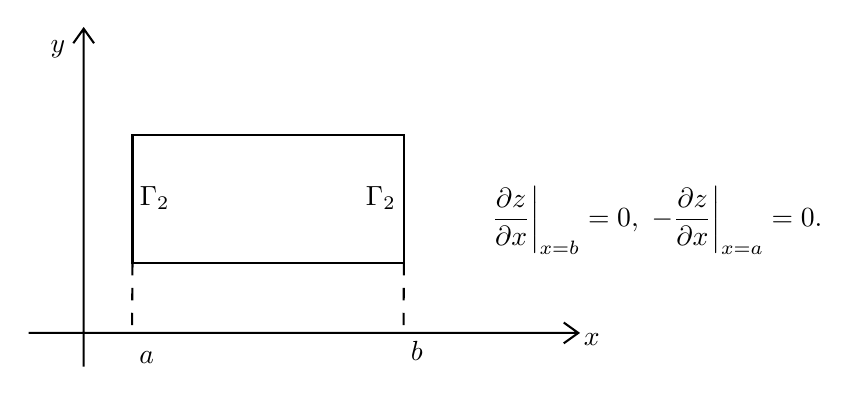
\begin{tikzpicture}[x=0.75pt,y=0.75pt,yscale=-1,xscale=1]
	%uncomment if require: \path (0,222); %set diagram left start at 0, and has height of 222
	
	%Shape: Axis 2D [id:dp7578165526074085] 
	\draw  (33,173.57) -- (297.78,173.57)(59.48,27) -- (59.48,189.85) (290.78,168.57) -- (297.78,173.57) -- (290.78,178.57) (54.48,34) -- (59.48,27) -- (64.48,34)  ;
	%Shape: Rectangle [id:dp16296921235920236] 
	\draw   (83,78) -- (213.78,78) -- (213.78,139.85) -- (83,139.85) -- cycle ;
	%Straight Lines [id:da6454278529068038] 
	\draw  [dash pattern={on 4.5pt off 4.5pt}]  (83,139.85) -- (82.78,172.85) ;
	%Straight Lines [id:da14183687134341394] 
	\draw  [dash pattern={on 4.5pt off 4.5pt}]  (213.78,139.85) -- (213.57,172.85) ;
	
	% Text Node
	\draw (299,172.4) node [anchor=north west][inner sep=0.75pt]    {$x$};
	% Text Node
	\draw (84.78,181.25) node [anchor=north west][inner sep=0.75pt]    {$a$};
	% Text Node
	\draw (215.57,176.25) node [anchor=north west][inner sep=0.75pt]    {$b$};
	% Text Node
	\draw (42,31.4) node [anchor=north west][inner sep=0.75pt]    {$y$};
	% Text Node
	\draw (85,101.4) node [anchor=north west][inner sep=0.75pt]    {$\Gamma _{2}$};
	% Text Node
	\draw (194,101.4) node [anchor=north west][inner sep=0.75pt]    {$\Gamma _{2}$};
	% Text Node
	\draw (253,101.4) node [anchor=north west][inner sep=0.75pt]    {$\displaystyle\left. \frac{\partial z}{\partial x}\right| _{x=b} =0,$};
	% Text Node
	\draw (330,101.4) node [anchor=north west][inner sep=0.75pt]    {$\displaystyle\left. -\frac{\partial z}{\partial x}\right| _{x=a} =0.$};
	
\end{tikzpicture}
	\caption{}
\label{l9:fig:4}
\end{figure}